% this file is called up by thesis.tex
% content in this file will be fed into the main document

%: ----------------------- name of chapter  -------------------------
\chapter{A Hybrid Gaussian-HMM-Deep-Learning Approach}\label{cp:ghmm} % top level followed by section, subsection


As recapped in Section~\ref{sec:2-rnnpm}, by now there are basically three types of deep learning approach for ACE:
\begin{itemize}
\item local classification - global smoothing \cite{humphrey2012rethinking};
\item local feature learning - global classification - global smoothing \cite{boulanger2013audio,sigtia2015audio};
\item local feature learning - local classification - global smoothing \cite{zhou2015chord}.
\end{itemize}
All these approaches apply similar deep learning methodologies in ASR \cite{deng2014deep,bourlard2012connectionist} directly to ACE, but they overlook a fundamental difference, that chords are usually segmented rhythmically and they are sustaining much longer than phonemes. This crucial divergence could allow some different approaches for ACE.

This chapter introduces a new approach that leverages this property of ACE. Particularly, the method described here can be categorized as ``local feature extraction - global segmentation - local classification'', which isolates the process of segmentation from classification, and only performs the latter within each segmented region. 

Note that in recent MIREX ACE submissions, systems' segmentation qualities are fairly comparable with each other \cite{burgoyne2014comparative}, and all these systems perform segmentation and classification in one single pass at the same time, which leads to the belief that setting apart the two will bring more benefit to system performance.

%: ----------------------- contents from here ------------------------

\section{System Framework} \label{sec:3-sysframe}

Figure~\ref{fig:3-sysover} depicts the ACE system framework considered in this chapter. The system training process is as follows:
\begin{enumerate}
\item Chroma features are extracted from each input track using a method similar to the one employed in the Chordino system~\cite{mauch2010automatic,cannam2010sonic} (elaborated in Section~\ref{sec:3-chordino-like fe}).
\item The feature sequence is then segmented (in terms of chords) by ground truth annotations.
\item Each feature segment is tiled into sub-segments (see Section~\ref{sec:3-seg-tile}).
\item The sub-segments, together with the segment's chord label, are then considered as one sample to train the deep learning model (described in detail in Section~\ref{sec:3-dlmodel}).
\item As for testing, the ground-truth segmentation process is replaced by a GMM-HMM segmentation process (Section~\ref{sec:3-chordino-like sg}).
\end{enumerate}


\begin{figure}
\centering
\includegraphics[width=0.5\columnwidth]{3/figures/sys.pdf}
\caption{GMM-HMM ACE System framework.}
\label{fig:3-sysover}
\end{figure}

\subsection{Feature Extraction} \label{sec:3-chordino-like fe}
Feature extraction starts by taking a raw input and resamples it at 11025 Hz, followed by transforming them using short-time-Fourier-transform (STFT) with 4096-point Hamming window and 512-point hop size. The process then proceeds to transform the linear-frequency-scale spectrogram (2049-bin) to log-frequency-scale (252-bin, 3 bins per semitone ranging from MIDI note 21 to 104), and tunes the spectrogram to standard tuning using equation~\ref{eq:2-tuning}. To enhance harmonic content and attenuate background noise, a standardization process is performed by running-mean subtraction and running-standard-deviation division along the frequency bins. This is followed by an NNLS method \cite{mauch2010approximate} (equation~\ref{eq:2-nnls}) to extract note activation patterns (84-bin, 1 bin per semitone). This matrix is further reduced to a 24-bin per column bass-treble chromagram weighted by the bass and treble profiles (Figure~\ref{fig:3-btprofile}). Each chroma in the chromagram is normalized by the maximum norm. Table~\ref{tab:3-felevels} provides a summary of different levels of features generated by this process.

\begin{figure}[htb]
\centering
\includegraphics[width=0.5\columnwidth]{3/figures/btp.pdf}
\caption{Bass(+) and treble(.) profiles.}
\label{fig:3-btprofile}
\end{figure}
% The bass profile is computed as a Rayleigh distribution in order to allow more high range salience to get in.

\begin{table}[htb]
\caption{Features extraction parameters.}
\centering
\footnotesize
\begin{tabular}{|c|c|c|} \hline
 Process & Output level & Bins \\ \hline
 STFT & spectrogram & 2049 \\ \hline
 Linear-Log Mapping & notegram & 252  \\ \hline
 Tuning & tuned notegram (-ns) & 252 \\ \hline
 NNLS & NNLS notegram (-nnls) & 84  \\ \hline
 Bass-treble Profiling & chromagram (-ch) & 24 \\ \hline
\end{tabular}
\label{tab:3-felevels}
\end{table}

Here are some simple showcases of the feature extraction process output at notegram level. All of them are extracted from acoustic piano audio.

Figure~\ref{fig:3-note_C} illustrates the notegram of a middle C note, Figure~\ref{fig:3-interval_CE} a major third interval built upon the middle C, and Figure~\ref{fig:3-chord_Cmaj} a C major chord rooted on the same note. Note the appearance of the harmonics and background noise.

\begin{figure}
\centering
\includegraphics[width=0.6\columnwidth]{3/figures/note_C.pdf}
\caption{Middle C note - notegram}
\label{fig:3-note_C}
\end{figure}

\begin{figure}
\centering
\includegraphics[width=0.6\columnwidth]{3/figures/interval_CE.pdf}
\caption{Major third interval - notegram}
\label{fig:3-interval_CE}
\end{figure}

\begin{figure}
\centering
\includegraphics[width=0.6\columnwidth]{3/figures/chord_Cmaj.pdf}
\caption{C major chord - notegram}
\label{fig:3-chord_Cmaj}
\end{figure}

The above are all simple music elements with pure pitches. Figure~\ref{fig:3-cp} is a notegram example of the intro (first few seconds) of {\it Let it be} . As this is just a piano intro, no vocal melody is involved. Note how it is rhythmically segmented.
\begin{figure}
\centering
\includegraphics[width=0.5\columnwidth]{3/figures/cp.png}
\caption{Chord progression example - notegram}
\label{fig:3-cp}
\end{figure}
Figure~\ref{fig:3-cpm} showcases a symmetrical example with vocal melody. It is extracted from the first line of the first verse. Note although this is much more corrupted, a rhythmical segmentation is also visually noticeable.
\begin{figure}
\centering
\includegraphics[width=0.5\columnwidth]{3/figures/cpm.png}
\caption{Chord progression with vocal melody example - notegram}
\label{fig:3-cpm}
\end{figure}

\newpage
\subsection{Segmentation} \label{sec:3-chordino-like sg}
Similar to \cite{cannam2013mirex}, the segmentation process is implemented as an expert knowledge driven GMM-HMM (as shown in Figure~\ref{fig:3-hmm1}), which is characterized as follows:
\begin{itemize}
\item The hidden node models discrete states of categorical chord classes.

\item The observable node represents continuous states of a chroma.

\item The emission probabilities are designed as a 24-dimension Gaussian distribution with parameters shown in Table~\ref{tab:3-gaussian}.

\item The transition matrix is set with a heavy uniform self-transition weight, which is more than 99 times of the uniform non-self-transition weight. 

\item The prior matrix is uniform.
\end{itemize}

\begin{table}
\caption{Segmentation parameters.}
\centering
\footnotesize
\begin{tabular}{|c|c|c|} \hline
      & $\mu$ & $\sigma^2$ \\ \hline
 Bass - chord bass & 1 & 0.1 \\ \hline
 Bass - not chord bass but chord note & 1 & 0.5  \\ \hline
 Bass - not bass & 0 & 0.1 \\ \hline
 Treble - chord note & 1 & 0.2  \\ \hline
 Treble - not chord note & 0 & 0.2 \\ \hline
 No Chord (for all notes)  & 1 & 0.2  \\ \hline
\end{tabular}
\label{tab:3-gaussian}
\end{table}

\begin{figure}[htb]
\centering
\includegraphics[width=0.4\columnwidth]{3/figures/hmm1.pdf}
\caption{GMM-HMM Segmentation.}
\label{fig:3-hmm1}
\end{figure}

Figure~\ref{fig:3-cdflow} summarizes the full information flow of the above feature extraction and segmentation process using the first line of {\it Let it be}. Note how representations are enhanced or compressed during this process.
\begin{figure}[h]
\centering
\includegraphics[width=1\columnwidth,angle =90]{3/figures/cdflow.pdf}
\caption{Information flow of feature extraction and segmentation}
\label{fig:3-cdflow}
\end{figure}

\subsection{Segment Tiling Process} \label{sec:3-seg-tile}

This process divides a segment into $N$ equal-sized sub-segments, and takes the average feature of each sub-segment, resulting in a $N$-frame segment. If the original number of frames is not divisible by $N$, the last frame is extended to make it divisible.

\subsection{Deep Learning Models} \label{sec:3-dlmodel}

Each $N$-frame segment is classified as a chord label through a deep learning model. Three types of model are considered: DBN, MLP, and RNN.

\subsubsection{Deep Belief Network}

The DBN, as shown in Figure~\ref{fig:3-dbn} models the chord posteriors conditioned on the tiled chromagram. In this model, the RBM formed by the input layer and the first hidden layer is a Gaussian-Bernoulli RBM because the input feature (chromagram) is in continuous value space. The RBMs formed by hidden layer pairs are Bernoulli-Bernoulli RBMs, since each neuron is stochastic binary \cite{hinton2006reducing}. In the fine-tuning phase, the network is regarded as a MLP and trained via SGD with back-propagation.

\begin{figure}[htb]
\centering
\includegraphics[width=0.4\columnwidth]{3/figures/dbn.pdf}
\caption{The deep belief network architecture used in our system. All layers are fully connected. The input is N-frame of features.}
\label{fig:3-dbn}
\end{figure}

\subsubsection{Multilayer Perceptrons}
The MLP model has the same bottom-up topology as the DBN model, but it is without the top-down generative connections. It is trained via SGD with back-propagation.

\subsubsection{Recurrent Neural Network}

The RNN shown in Figure~\ref{fig:3-rnn} is bidirectional with LSTM hidden units \cite{hochreiter1997long}, or it can be called a BLSTM-RNN. As recapped in chapter~\ref{cp:background}, LSTM is introduced in order to relief gradient vanishing/exploding problem for long sequence training \cite{bengio2009learning}. For a fixed length $N$-frame input, the RNN is expanded to $N$ frames, each taking one frame of input. A mean pooling operation \cite{maas2011learning}, similar to those normally used in a CNN \cite{lecun1995convolutional}, is inserted before the output layer to summarize the LSTM activations of all frames.
\begin{figure}[h]
\centering
\includegraphics[width=0.6\columnwidth]{3/figures/rnn.pdf}
\caption{The bidirectional recurrent neural network architecture used in our system. Both hidden layers employ LSTM units in place of normal logistic units. The RNN is expanded to N frames, with mean pooling to summarize results.}
\label{fig:3-rnn}
\end{figure}

\section{Experiments} \label{sec:3-exper}
This section describes a systematic approach to sample the design space of the ACE framework. All system configurations are tested under the same benchmark. %First the datasets is introduced, and then the design space sampling scheme is elaborated. This section is ended by expounding the training and testing process.

\subsection{Datasets}
For training/validation, five datasets of 366 tracks in total is used. They contain both eastern and western pop/rock songs. They are:
\begin{enumerate}
\item JayChou29 (J) dataset \cite{deng2016chord}, annotated by the author of this thesis\footnote{\url{http://www.tangkk.net/label/}};
\item a Chinese pop song dataset (CNPop20, or C)\footnote{containing 20 songs from both male and female singer-songwriters from Chinese cultural backgrounds}, also annotated by the author \cite{deng2016hybrid};
\item Carole King + Queen dataset (KingQueen26, or K)\footnote{\url{http://isophonics.net/datasets}}, annotated by Mauch \cite{mauch2009omras2} in C4DM (Center for Digital Music in Queen Mary University of London);
\item 191 songs from USPop dataset (U)\footnote{\url{http://labrosa.ee.columbia.edu/projects/musicsim/uspop2002.html}}, annotated by MARL (Music and Audio Research Lab in New York University)\footnote{\url{https://github.com/tmc323/Chord-Annotations}} \cite{cho2014improved};
\item 100 songs from RWC dataset, provided by the RWC group\footnote{\url{https://staff.aist.go.jp/m.goto/RWC-MDB/}} and also annotated by MARL \cite{cho2014improved}.
\end{enumerate}


Each track is extracted at both -ns and -ch level. They are transposed to all 12 different keys by circular pitch shifting (for -ch) or pitch shifting with zero padding (for -ns). Adjusting the ground truth labels accordingly, this results in a 12-time data augmentation, which helps in reducing over-fitting \cite{cho2014improved,humphrey2015exploration}. This is commonly considered as a type of regularization.

Combination of datasets is notated by concatenating their letter codes. For example, a combination of all training datasets is denoted as ``CJKU''. These notations will be used extensively in Section~\ref{sec:3-res}.

For testing, we use TheBeatles180 (B) dataset, annotated by Harte \cite{harte2010towards}, who refers to Pollack's previous chord transcriptions \cite{pollack2000notes}. This can be regarded as a benchmarking dataset that measures how well a system generalizes outside the scope of data that it has been trained on.

\subsection{Design Space Sampling}
There is a large design space under the system framework. Specifically, possible dimensions include:
\begin{itemize}
\item choice of deep learning model; 
\item depth and width of hidden layers (network configurations);
\item number of frames in segment tiling;
\item input feature representation level; and
\item training data size.
\end{itemize}

\begin{table}
\caption{Variations considered in this study.}
\centering
\footnotesize
\begin{tabular}{|c|c|c|} \hline
Dimension & Configurations to Try \\ \hline
model & MLP; DBN; BLSTM-RNN \\ \hline
N-frame & 1; 2; 3; 6; 9; 12 \\ \hline
layer depth & 2; 3; 4; 5 \\ \hline
layer width & 500; 800; 1000; 2000 \\ \hline
input representation & tuned notegram (-ns); chromagram (-ch) \\ \hline
training data size & J; CJK; CJKU \\ \hline
\end{tabular}
\label{tab:3-varexplore}
\end{table}

This study is based on the settings depicted in Table~\ref{tab:3-varexplore}. Indeed, it is impractical to sample all combinations. A more practical yet systematic method is proposed, which samples one dimension at a time with all other dimensions fixed at a previously explored point. If a dimension is not yet explored, a random choice of value is used.

Specifically, the scheme first samples along the {\it layer width}, and then along the {\it layer depth}. After understanding the two variations, we explore the $N$-frame with fixed {\it layer width} and {\it layer depth}. Following this same strategy, all factors in Table~\ref{tab:3-varexplore} are explored. It is important to note that neither does this process lead to a full picture of the design space, nor does it lead to optimality, but it gains us general insights.

%The concrete samples and their performances will be discussed in Section \ref{sec:3-res}.

\subsection{Training and Testing}

To control variations of training, we apply the following techniques in all implementations. 
\begin{itemize}
\item An MLP model is trained using mini-batch stochastic gradient descent regularized with dropout \cite{srivastava2014dropout} and early-stopping \cite{prechelt1998automatic}. 
\item A DBN model is pre-trained using persistent-contrastive-divergence \cite{tieleman2008training} (PCD-20), for 100 epochs with learning rate 0.001. It is fine-tuned using mini-batch stochastic gradient descent regularized with dropout and early-stopping.
\item During mini-batch stochastic gradient descent, both MLP and DBN use a learning rate of 0.01 and a batch size of 100. 
\item A BLSTM-RNN model is trained using an Adadelta optimizer \cite{zeiler2012adadelta}, regularized with dropout and early-stopping. 
\item All dropout probabilities are set to 0.5. 
\item The early-stopping event is cross-checked by a validation set, which is a random choice of 20\% of the training dataset, while the other 80\% are used for computing gradients and updating the network.
\end{itemize}

One interesting observation in this study is that randomness incorporated in the original design does not really provide significant flexibility in training data selection and model initialization. Indeed, through extensive experiments, specifically those described in Section~\ref{sec:3-res}, it can be found that randomness in the system only contributes to very limited amount of unpredictability, leading to rather minimal impact on the general exploration of design space. Moreover, the strong regularities provided by data augmentation, generative pre-training, and other techniques, more or less offset the randomness effect during training/validation split.

In the testing process, each of the 180 tracks in the test dataset are chord estimated from raw audio file. The output is written in a {\tt .lab} file conforming with the ``start\_time end\_time chord'' format\footnote{\url{http://www.music-ir.org/mirex/wiki/2016:Audio\_Chord\_Estimation}}, where the ``chord'' is conforming with Harte's format \cite{harte2005symbolic}. All implementation details are available online\footnote{\url{github.com/tangkk/tangkkace}} in so that interested readers can repeat the experiments. All deep learning components are implemented under the framework of Theano \cite{bergstra2010theano}.

\section{Results and Discussions} \label{sec:3-res}
% explain the WCSR metric 
% explain the Baseline

% systematic sampling from the whole design space of this hybrid approach (common variations)
% - DBN-ch robust to layer width and layer depth
% - DBN-ns NOT robust to network configurations; better with 2-3 hidden layers (e.g. [800,800]), regardless of layer width
% - MLP not stable with different N-frame; DBN is stable with different N-frame; BLSTM-RNN performs better with larger N.
% - System performs better at chromagram level (ch) and than tuned notegram level (ns)
% - At ch level, both MLP and DBN are robust to training data size, while BLSTM-RNN benefits from more data
% - At ns level, both MLP and BLSTM-RNN benefit from more data, while DBN is still robust to data size
% - BLSTM does better on long-tail chords, while both MLP and DBN tends to over-fit dominant chords

% using pdfplots (https://www.sharelatex.com/learn/Pgfplots_package) to plot the data as categorical bar plots or line chart, with ymin = 0, ymax = 100
% show only the SeventhsBass result
% add a plot showing all MIREX vocabulary results comparing the two best system with the baseline
% talk about confusions relationships of Mm, MmB, S, SB...
% showing Mm/SB, MmB/SB, S/SB (talking about the ratio mean, std, and possibly a curve), using a box plot to compress message), taking all relevant systems into separate consideration. This justifies why only showing SB's results.

%This section reveals design space regularities, which are indicated by several insights derived from the experiment results. Throughout the section, we title each subsection with a summary of the insight before discussing the results. 
%Before heading into the evaluation details, we need to define the evaluation metric.

Throughout this section, the current MIREX ACE standard evaluation metrics (as reviewed in Section~\ref{sec:2-eval}) will be used to report system performances. Unless otherwise specified, the following WCSR scores are all reported under SeventhsBass evaluation, where a correct classification does {\it not} involve any chord mapping scheme beyond SeventhsBass vocabulary \cite{pauwels2013evaluating,burgoyne2014comparative}.

Apart from exploration, the best system variants are also compared with Chordino\footnote{\url{http://www.isophonics.net/nnls-chroma}} \cite{cannam2010sonic}. It should be noted that Chordino represents the best benchmark because: (1) Our framework resembles Chordino's in terms of segmentation and feature extraction; (2) Chordino is the only other system that supports large vocabulary as well as chord inversions.

%The analysis also generally applies to other vocabulary subsets, because under our system framework, WCSRs of SeventhsBass is steadily in proportion to WCSRs of MajMin, MajMinBass and Sevenths (elaborated in Section \ref{sec:3-p8}). 
\subsection{Intra-comparison and Implications}
\Hsection{DBN-ns with 2 hidden layers performs at least as good as a deeper model; Layer width plays a minor role} \label{sec:3-p1}

\pgfplotsset{width=8cm,height=4cm,every node near coord/.append style={font=\scriptsize}}
\begin{figure}[htb]
\centering
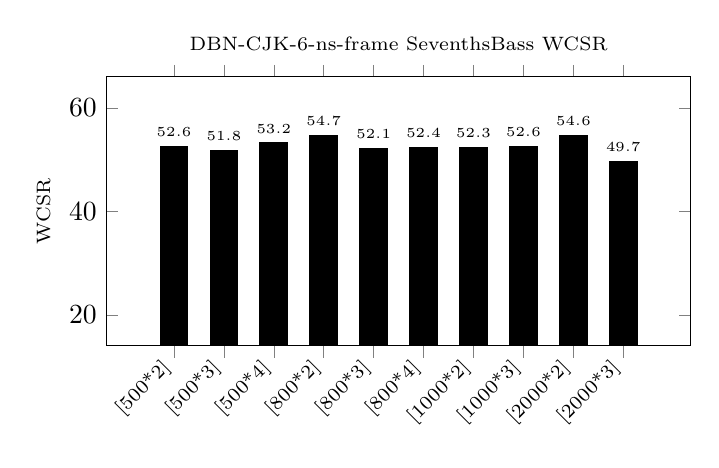
\begin{tikzpicture}
\begin{axis}[
	title=DBN-CJK-6-ns-frame SeventhsBass WCSR,
	title style = {font=\scriptsize},
    ybar,
    enlargelimits=0.15,
        legend style={at={(0.5,-0.3)},
          anchor=north,legend columns=-1},
    ylabel={WCSR},
    y label style={font=\scriptsize},
    symbolic x coords={[500*2],[500*3],[500*4],[800*2],[800*3],[800*4],[1000*2],[1000*3],[2000*2],[2000*3]},
    x tick label style={rotate=45,anchor=east, font=\scriptsize},
    xtick=data,
    ymin=20, ymax=60,
    nodes near coords,
    nodes near coords align={vertical},
    ]
\addplot [fill=black,draw=black] coordinates {([500*2],52.6)([500*3],51.8)([500*4],53.2)([800*2],54.7)([800*3],52.1)([800*4],52.4)([1000*2],52.3)([1000*3],52.6)([2000*2],54.6)([2000*3],49.7)};
\end{axis}
\end{tikzpicture}
\caption{Exploring different DBN-ns network configurations. All systems are trained with CJK-6-ns-frame.}
\label{fig:3-dbn-ns-configs}
\end{figure}

Figure~\ref{fig:3-dbn-ns-configs} shows the scores of ten DBN-ns systems with different network configurations. They have 2, 3 or 4 hidden layers with 500, 800, 1000 or 2000 layer width. A major observation is that [800*2] achieves the best score, followed by [2000*2], and the difference between the highest and the lowest score is 5 points.

The results indicate that, in terms of DBN-ns systems, a two-hidden-layer network generally performs better than or at least as good as a deeper architecture with the same layer width. Because these systems are all trained using CJK, a plausible implication is that more data will help train a better system for a deeper architecture, but as will soon be discussed in Section~\ref{sec:3-p6}, DBN-ns is indeed very impervious to training data size.%We will come back to this in that Section.

\Hsection{DBN-ch is robust to both layer width and layer depth} \label{sec:3-p2}

\pgfplotsset{width=8cm,height=4cm,every node near coord/.append style={font=\scriptsize}}
\begin{figure}[htb]
\centering
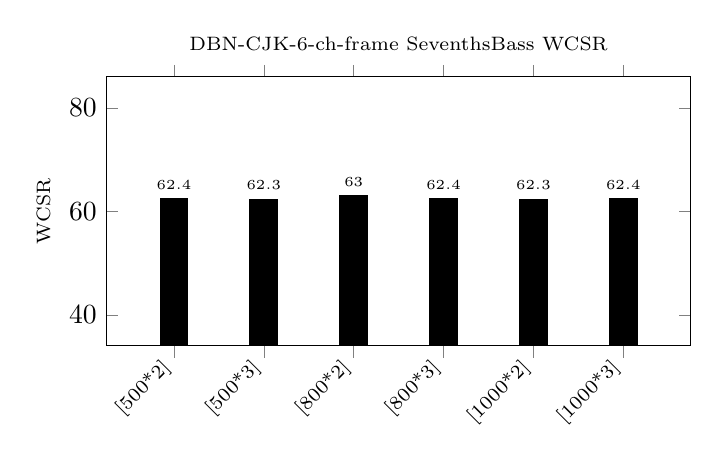
\begin{tikzpicture}
\begin{axis}[
	title=DBN-CJK-6-ch-frame SeventhsBass WCSR,
	title style = {font=\scriptsize},
    ybar,
    enlargelimits=0.15,
        legend style={at={(0.5,-0.3)},
          anchor=north,legend columns=-1},
    ylabel={WCSR},
    y label style={font=\scriptsize},
    symbolic x coords={[500*2],[500*3],[800*2],[800*3],[1000*2],[1000*3]},
    x tick label style={rotate=45,anchor=east, font=\scriptsize},
    xtick=data,
    ymin=40, ymax=80,
    nodes near coords,
    nodes near coords align={vertical},
    ]
\addplot [fill=black,draw=black] coordinates {([500*2],62.4)([500*3],62.30)([800*2],63.0)([800*3],62.4)([1000*2],62.3)([1000*3],62.4)};
\end{axis}
\end{tikzpicture}
\caption{Exploring different DBN-ch network configurations. All systems are trained with CJK-6-ch-frame.}
\label{fig:3-dbn-ch-configs}
\end{figure}

Figure~\ref{fig:3-dbn-ch-configs} shows scores of DBN-ch systems with different network configurations. Ranging from 62.3 to 63, they are all close to each other, which demonstrates that DBN-ch is robust to network configurations, given a reasonable amount of modeling capacity.

%despite the moderate variation of network configurations similar to those of Section \ref{sec:3-p1}

Considering both Sections~\ref{sec:3-p1} and~\ref{sec:3-p2}, it can be credibly deduced that DBN-ch is more robust than DBN-ns in terms of network configurations. Given that they both peak at [800*2] (also denoted as (800,800) in the following), this configuration is chosen as a default for most of the following experiments without consulting the optimality, which in general is not a central issue throughout this discussion.

\Hsection{MLP is susceptible to N-frame; DBN is impervious to N-frame; BLSTM-RNN generally performs better with larger N} \label{sec:3-p3}

\pgfplotsset{width=8cm,height=4cm,every node near coord/.append style={font=\scriptsize}}
\begin{figure}
\centering
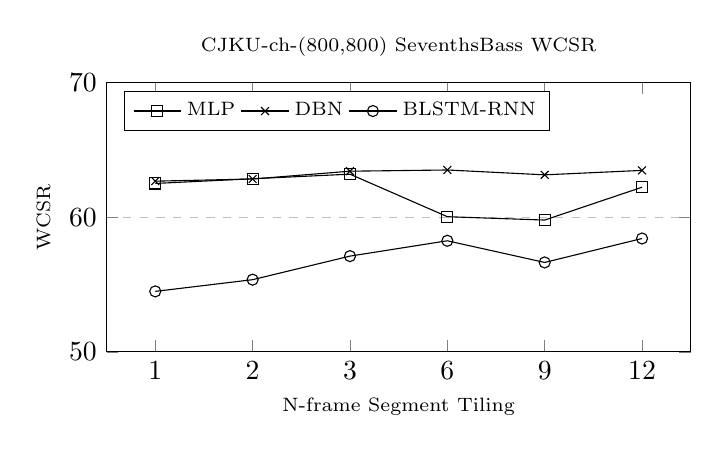
\begin{tikzpicture}
\begin{axis}[
    title={CJKU-ch-(800,800) SeventhsBass WCSR},
    title style = {font=\scriptsize},
    xlabel={N-frame Segment Tiling},
    x label style={font=\scriptsize},
    ylabel={WCSR},
    y label style={font=\scriptsize},
    ymin=50, ymax=70,
    symbolic x coords={1,2,3,6,9,12},
    ytick={50,60,70},
    legend pos=north west,
    legend style={legend columns=-1, font=\scriptsize},
    ymajorgrids=true,
    grid style=dashed,
]
 
\addplot[
    color=black,
    mark=square,
    ]
    coordinates {
    (1,62.51)(2,62.86)(3,63.20)(6,60.04)(9,59.79)(12,62.23)
    };
    
\addplot[
    color=black,
    mark=x,
    ]
    coordinates {
    (1,62.68)(2,62.84)(3,63.42)(6,63.51)(9,63.15)(12,63.48)
    };
    
 \addplot[
     color=black,
     mark=o,
     ]
     coordinates {
     (1,54.49)(2,55.36)(3,57.11)(6,58.25)(9,56.64)(12,58.42)
     };
\legend{MLP, DBN, BLSTM-RNN} 
\end{axis}
\end{tikzpicture}
\caption{Exploring effect of N-frame. All systems are trained with CJKU-ch-(800,800)}
\label{fig:3-N-frame}
\end{figure}

A set of systems are implemented using CJKU-ch-(800,800) with different $N$-frame segment tiling. The (800,800) in BLSTM-RNN means there are one forward and one backward hidden layer, each having 800 LSTM units.

As depicted in Figure~\ref{fig:3-N-frame}, MLP is not stable with the change of $N$. Being fully connected, it does not exploit the input in any predefined order. Consequently, given inputs of different number of frames, it may learn them in different ways, leading to uncertain trend of the results. However, as for DBN, the scores stay steadily between 62 and 63. This is due to the generative pre-training that regularizes the network and thus minimizes the difference of segment tiling.

%As depicted in Figure~\ref{fig:3-N-frame}, DBN stays steadily around 62 and 63. Being fully connected, DBN is good at general classification, which does not exploit the input in any predefined order. It tends to regard every frame equally as if the order is not important. Although in ACE the order of frames does convey meanings, DBN tends to ignore or weaken them, which possibly explains why it is impervious to $N$.

%However, although MLP is also exploiting space dependency, it is not as robust to $N$ as DBN does. Without generative pre-training, it lacks a self-regularized mechanism to adapt to changes in input representation, leading to a somewhat unstable behavior with regard to $N$.

%But generally, with smaller $N$, the ``order'' information within the input is better summarized

%This may be caused by the much weaker regularization in its training process, leading to a somewhat volatile model with a random split of training/validation set.

As for BLSTM-RNN, though it has a local maximum at $N=3$, it tends to perform better with larger $N$. RNN is best for exploiting temporal dependencies within input features. It strongly relates frames to each other according to their order. This explains why it scores better with finer-grain tiling.

As optimality is not the main focus, without any bias towards $N$, we choose $N=6$ as a default for further experiments.

\Hsection{MLP and DBN generally perform better at -ch level than at -ns level; For BLSTM-RNN, the opposite is true}\label{sec:3-p4}

\begin{figure}[htb]
\centering
\pgfplotsset{width=8cm,height=4cm,every node near coord/.append style={font=\scriptsize}}
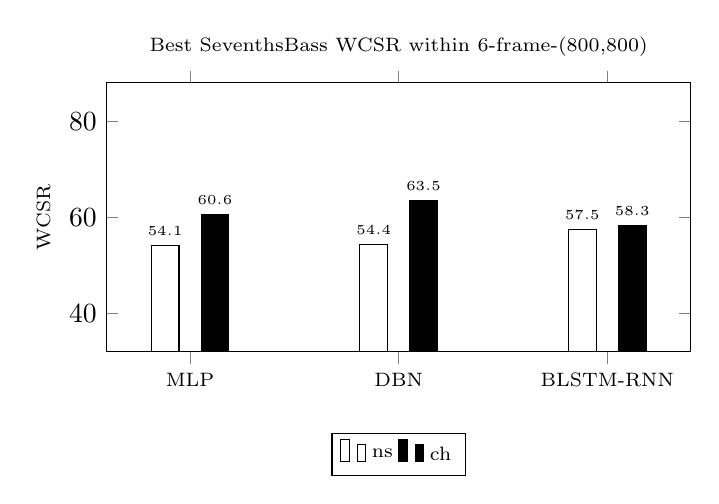
\begin{tikzpicture}
\begin{axis}[
	title={Best SeventhsBass WCSR within 6-frame-(800,800)},
	title style = {font=\scriptsize},
    ybar=8pt,
    enlargelimits=0.2,
        legend style={at={(0.5,-0.3)},
          anchor=north,legend columns=-1},
    ylabel={WCSR},
    y label style={font=\scriptsize},
    symbolic x coords={MLP,DBN,BLSTM-RNN},
    x tick label style={font=\scriptsize},
    xtick=data,
    ymin=40, ymax=80,
    nodes near coords,
    nodes near coords align={vertical},
    legend style={font=\scriptsize},
    ]
\addplot [ybar,fill=white,draw=black] coordinates {(MLP,54.1)(DBN,54.4)(BLSTM-RNN,57.5)};
\addplot [ybar,fill=black,draw=black] coordinates {(MLP,60.6)(DBN,63.5)(BLSTM-RNN,58.3)};
\legend{ns,ch}
\end{axis}
\end{tikzpicture}
\caption{Exploring input feature levels. All systems are trained with 6-frame-(800,800)}
\label{fig:3-ns-ch}
\end{figure}

To analyze effect of input representation level, for each deep learning model we train several 6-frame-(800,800) systems on both -ns and -ch level using different combination of datasets from J to CJKU. The best scores in each category are reported in Figure~\ref{fig:3-ns-ch}.

%Figure \ref{fig:3-ns-ch} shows six best scores of 6-frame-(800,800) systems, which summarize scores of all such systems trained with different combination of datasets from J to CJKU.

For MLP and DBN, systems at -ch level performs much better than those at -ns level. This is on one hand due to the fact that the feature extraction process from tuned notegram to chromagram musically makes sense, and on the other hand owing to the completeness deficiency of all MLP-ns and DBN-ns models. These models fail to transform data as nicely as handcrafted transformations, even with deeper models (refer to Section~\ref{sec:3-p1}) or more data (will be elaborated in Section~\ref{sec:3-p6}).

This points to an interesting fact that these deep models could not learn as much regularities from the data as human beings do given the stated training process. The dominating factor behind this reasonably would be that they both tend to spend too much budget looking for regularities that are cross-frame and time irrelevant.
%Actually, their input is a concatenation of N-frame into one single vector, which does not even have a clue of ``time''.

On the contrary, BLSTM-RNN-ns generally scores better than the BLSTM-RNN-ch. Unlike MLP and DBN, RNN has a natural structure of modeling temporal dependency. Consequently, under an ACE task with the same resource constraint, it learns more meaningful regularities in time dimension. But due to transformations from -ns to -ch, some originally presented regularities are missing or destroyed, such as the distribution and continuation of absolute pitch saliences. This explains why BLSTM-RNN achieves better scores at -ns than at -ch level.

%Thus there is less evidence to learn from, which gives rise to lower scores.

%That's why it achieves good results at -ns level. However, at -ch level, 
%This reflects the advantage of deep learning, that a system benefits more by starting from deeper level of representations (closer to raw level input). This is supported by an argument that handcrafted features are usually suboptimal, and optimality could only be attained by learning from data at raw representation level.

%where the fine detail of a chord is generally lost

Note that at -ch level BLSTM-RNN's performance is generally worse than those of MLP and DBN. While BLSTM-RNN tries to explore useful information related to time, MLP and DBN try to search in terms of space. As chromagram is already a summary of notegram, searching regularities in an order-irrelevant style is economic and effective. To learn a function from chromagram to chord label could be as easy as spotting the relative salience undulations across frames. But this order-irrelevant learning process sometimes overlooks the fine details that distinguish a ordinary chord\footnote{chords with majority population, not to be confused with its other meanings} from a long-tail chord\footnote{chords with minority population}. For example, it may overlook the difference between $maj$ and $maj/3$. Therefore, albeit efficient, it could easily over-fit ordinary chords, or under-fit long-tail chords, which are susceptible to confusion with ordinary chords. This over-fitting phenomenon is confirmed by our experiment in Section~\ref{sec:3-p7}.

\Hsection{At -ch level, both MLP and DBN are impervious to training data size, while BLSTM-RNN benefits from more training data}\label{sec:3-p5}

\begin{figure}[htb]
\centering
\pgfplotsset{width=8cm,height=4cm,every node near coord/.append style={font=\scriptsize}}
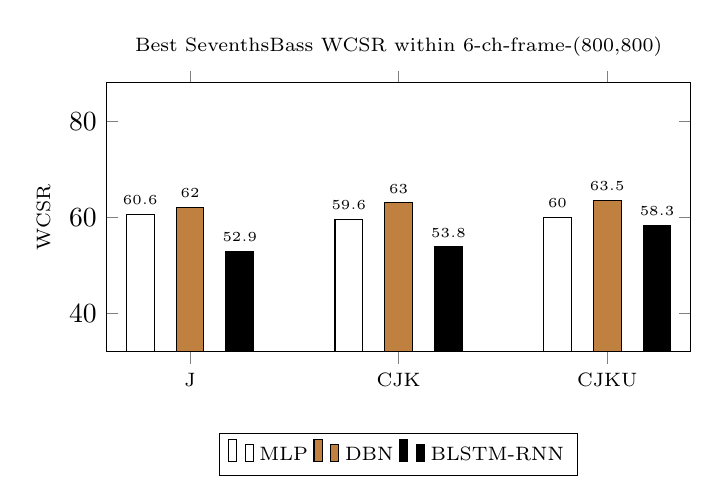
\begin{tikzpicture}
\begin{axis}[
	title={Best SeventhsBass WCSR within 6-ch-frame-(800,800)},
	title style = {font=\scriptsize},
    ybar=8pt,
    enlargelimits=0.2,
        legend style={at={(0.5,-0.3)},
          anchor=north,legend columns=-1},
    ylabel={WCSR},
    y label style={font=\scriptsize},
    symbolic x coords={J,CJK,CJKU},
    x tick label style={font=\scriptsize},
    xtick=data,
    ymin=40, ymax=80,
    nodes near coords,
    nodes near coords align={vertical},
    legend style={font=\scriptsize},
    ]
\addplot [ybar,fill=white,draw=black] coordinates {(J,60.6)(CJK,59.6)(CJKU,60.0)};
\addplot [ybar,fill=brown,draw=black] coordinates {(J,62.0)(CJK,63.0)(CJKU,63.5)};
\addplot [ybar,fill=black,draw=black] coordinates {(J,52.9)(CJK,53.8)(CJKU,58.3)};
\legend{MLP,DBN,BLSTM-RNN}
\end{axis}
\end{tikzpicture}
\caption{Exploring different training data size at -ch level. All systems are trained with 6-ch-frame-(800,800).}
\label{fig:3-ch-data}
\end{figure}

Both this and the next subsections examine the effect of training data size on different deep learning models. At -ch level, the results in Figure \ref{fig:3-ch-data} show that both MLP and DBN are impervious to training data size, while BLSTM-RNN performs better with more data.

As mentioned in the previous subsection, MLP and DBN are naturally suitable to this task as they only look for relative salience regularities in different frames and build up simple connections to chord labels. As a result, even with small amount of training data the models are still able to learn meaningful but probably ``over-fitting-prone'' classification rules.

%, such as J, which contains 29 tracks with around 1000 chord cases,
%Since at -ch level the chromagram has already contained very strong prior regarding the harmonic structure of the input, the remaining step to be learned is the pitch class saliences summarization process.

As for BLSTM-RNN, it pays too much attention to look for time-related regularities, thus sacrificing the ``easy way out''. But under ACE context, leveraging ``time-related'' regularities to recognize chords makes sense musically. Thus, BLSTM-RNN makes steady progress with more training data.

\Hsection{At -ns level, DBN is still impervious to training data size, while both MLP and BLSTM-RNN benefit from more training data}\label{sec:3-p6}

\begin{figure}[htb]
\centering
\pgfplotsset{width=8cm,height=4cm,every node near coord/.append style={font=\scriptsize}}
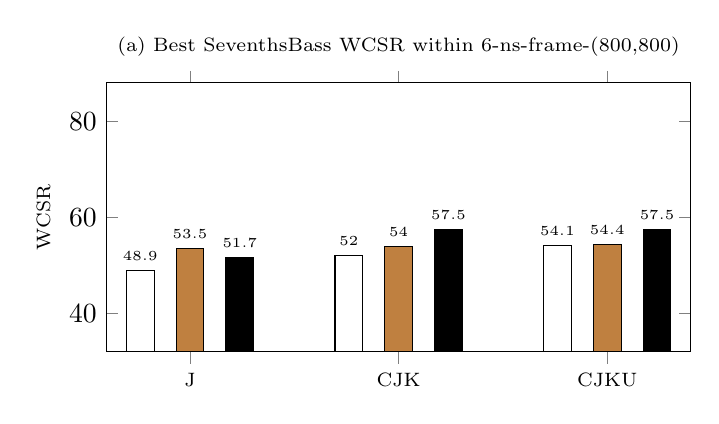
\begin{tikzpicture}
\begin{axis}[
	title={(a) Best SeventhsBass WCSR within 6-ns-frame-(800,800)},
	title style = {font=\scriptsize},
    ybar=8pt,
    enlargelimits=0.2,
        legend style={at={(0.5,-0.3)},
          anchor=north,legend columns=-1},
    ylabel={WCSR},
    y label style={font=\scriptsize},
    symbolic x coords={J,CJK,CJKU},
    x tick label style={font=\scriptsize},
    xtick=data,
    ymin=40, ymax=80,
    nodes near coords,
    nodes near coords align={vertical},
    legend style={font=\scriptsize},
    ]
\addplot [ybar,fill=white,draw=black] coordinates {(J,48.9)(CJK,52.0)(CJKU,54.1)};
\addplot [ybar,fill=brown,draw=black] coordinates {(J,53.5)(CJK,54.0)(CJKU,54.4)};
\addplot [ybar,fill=black,draw=black] coordinates {(J,51.7)(CJK,57.5)(CJKU,57.5)};
%\legend{MLP,DBN,BLSTM-RNN}
\end{axis}
\end{tikzpicture}
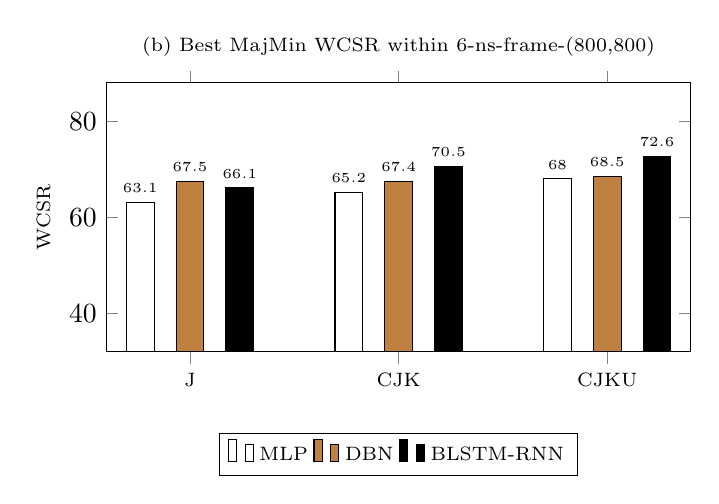
\begin{tikzpicture}
\begin{axis}[
	title={(b) Best MajMin WCSR within 6-ns-frame-(800,800)},
	title style = {font=\scriptsize},
    ybar=8pt,
    enlargelimits=0.2,
        legend style={at={(0.5,-0.3)},
          anchor=north,legend columns=-1},
    ylabel={WCSR},
    y label style={font=\scriptsize},
    symbolic x coords={J,CJK,CJKU},
    x tick label style={font=\scriptsize},
    xtick=data,
    ymin=40, ymax=80,
    nodes near coords,
    nodes near coords align={vertical},
    legend style={font=\scriptsize},
    ]
\addplot [ybar,fill=white,draw=black] coordinates {(J,63.1)(CJK,65.2)(CJKU,68.0)};
\addplot [ybar,fill=brown,draw=black] coordinates {(J,67.5)(CJK,67.4)(CJKU,68.5)};
\addplot [ybar,fill=black,draw=black] coordinates {(J,66.1)(CJK,70.5)(CJKU,72.6)};
\legend{MLP,DBN,BLSTM-RNN}
\end{axis}
\end{tikzpicture}
\caption{Exploring training data size at -ns level. All systems are trained with 6-ns-frame-(800,800).}
\label{fig:3-ns-data}
\end{figure}

At -ns level, as shown in Figure~\ref{fig:3-ns-data}, with more training data, DBN still exhibits similar performances, but both MLP and BLSTM-RNN performs better. Interestingly, BLSTM-RNN does not show any improvement in terms of SeventhsBass WCSR moving from CJK to CJKU, but does have a lot improvement in MajMin (Figure~\ref{fig:3-ns-data} (b)). MajMin WCSR is calculated by accepting two types of chord confusions based on SeventhsBass WCSR (relationships between all vocabularies in MIREX ACE evaluation will be discussed in Section~\ref{sec:3-p8}).

%Unlike chromagram, the tuned notegram at -ns level does not imply a prior that strongly indicates the harmonic structure of the underlying chord, hence both MLP and DBN struggle to search for regularities to relate these raw information to chord labels. However, BLSTM-RNN may find this material easier to learn since it contains a lot more time-related clue for chord prediction. Under this circumstance, it is foreseeable that MLP and BLSTM-RNN performs better with more data. As for DBN, it is pre-trained as a generative model using unlabeled data before trained as a discriminative model using labeled data. The generative pre-training theoretically makes the model generalize better compared with the same model without pre-training \cite{hinton2006fast}. The fact that DBN maintains similar performances across all three training datasets echoes with this theory.

\Hsection{BLSTM-RNN recognizes much better on long-tail chords, while MLP and DBN tend to over-fit ordinary chords}\label{sec:3-p7}
\begin{figure*}[htb]
\centering
\pgfplotsset{width=15cm,height=4cm,every node near coord/.append style={font=\scriptsize}}
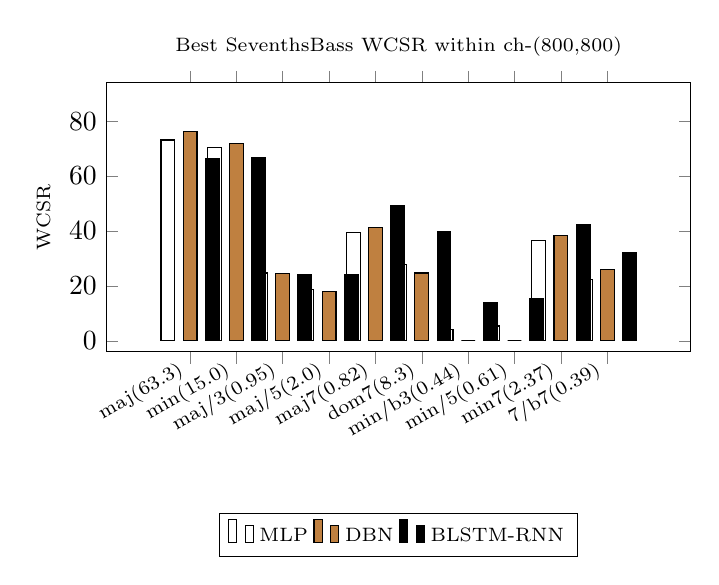
\begin{tikzpicture}
\begin{axis}[
	title={Best SeventhsBass WCSR within ch-(800,800)},
	title style = {font=\scriptsize},
    ybar=3pt,
    bar width=5pt,
    enlargelimits=0.2,
        legend style={at={(0.5,-0.6)},
          anchor=north,legend columns=-1},
    ylabel={WCSR},
    y label style={font=\scriptsize},
    symbolic x coords={maj(63.3), min(15.0), maj/3(0.95), maj/5(2.0), maj7(0.82), dom7(8.3), min/b3(0.44), min/5(0.61), min7(2.37), 7/b7(0.39)},
    x tick label style={rotate=30,anchor=east, font=\scriptsize},
    xtick=data,
    ymin=10, ymax=80,
    %nodes near coords,
    nodes near coords align={vertical},
    legend style={font=\scriptsize},
    ]
\addplot [ybar,fill=white,draw=black] coordinates {(maj(63.3),73.1)(min(15.0),70.3)(maj/3(0.95),24.7)(maj/5(2.0),18.7)(maj7(0.82),39.3)(dom7(8.3),27.8)(min/b3(0.44),4.2)(min/5(0.61),5.4)(min7(2.37),36.6)(7/b7(0.39),22.2)};

\addplot [ybar,fill=brown,draw=black] coordinates {(maj(63.3),76.3)(min(15.0),71.7)(maj/3(0.95),24.6)(maj/5(2.0),18.1)(maj7(0.82),41.3)(dom7(8.3),24.7)(min/b3(0.44),0)(min/5(0.61),0)(min7(2.37),38.3)(7/b7(0.39),25.9)};

\addplot [ybar,fill=black,draw=black] coordinates {(maj(63.3),66.2)(min(15.0),66.6)(maj/3(0.95),24.0)(maj/5(2.0),24.3)(maj7(0.82),49.1)(dom7(8.3),39.7)(min/b3(0.44),13.9)(min/5(0.61),15.4)(min7(2.37),42.2)(7/b7(0.39),32.0)};

\legend{MLP,DBN,BLSTM-RNN}
\end{axis}
\end{tikzpicture}
\caption{Different models' handling of long-tail and ordinary chords. All systems are trained with ch-(800,800). Numbers in brackets indicates the percentage of chord within the test set.}
\label{fig:3-blstm-long-tail}
\end{figure*}

\begin{figure}[htb]
\centering
\pgfplotsset{width=6cm,height=4cm,every node near coord/.append style={font=\scriptsize}}
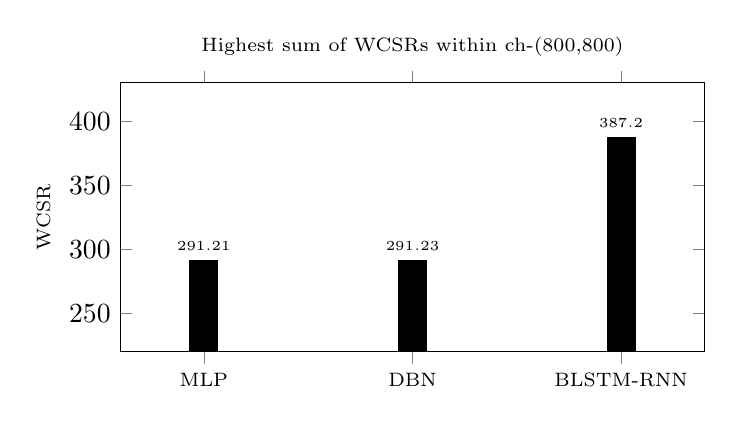
\begin{tikzpicture}
\begin{axis}[
	title={Highest sum of WCSRs within ch-(800,800)},
	title style = {font=\scriptsize},
    ybar=8pt,
    enlargelimits=0.2,
        legend style={at={(0.5,-0.3)},
          anchor=north,legend columns=-1},
    ylabel={WCSR},
    y label style={font=\scriptsize},
    symbolic x coords={MLP,DBN,BLSTM-RNN},
    x tick label style={font=\scriptsize},
    xtick=data,
    ymin=250, ymax=400,
    nodes near coords,
    nodes near coords align={vertical},
    legend style={font=\scriptsize},
    ]
\addplot [ybar,fill=black,draw=black] coordinates {(MLP,291.21)(DBN,291.23)(BLSTM-RNN,387.2)};
\end{axis}
\end{tikzpicture}
\caption{Sum of WCSRs in all SeventhsBass Chord Categories. All systems are trained with ch-(800,800).}
\label{fig:3-sumofsb}
\end{figure}

\begin{figure}[htb]
\centering
\pgfplotsset{width=6cm,height=4cm,every node near coord/.append style={font=\scriptsize}}
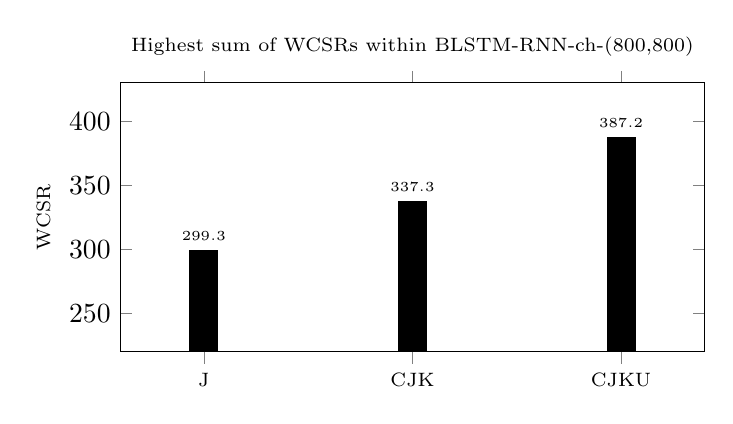
\begin{tikzpicture}
\begin{axis}[
	title={Highest sum of WCSRs within BLSTM-RNN-ch-(800,800)},
	title style = {font=\scriptsize},
    ybar=8pt,
    enlargelimits=0.2,
        legend style={at={(0.5,-0.3)},
          anchor=north,legend columns=-1},
    ylabel={WCSR},
    y label style={font=\scriptsize},
    symbolic x coords={J,CJK,CJKU},
    x tick label style={font=\scriptsize},
    xtick=data,
    ymin=250, ymax=400,
    nodes near coords,
    nodes near coords align={vertical},
    legend style={font=\scriptsize},
    ]
\addplot [ybar,fill=black,draw=black] coordinates {(J,299.3)(CJK,337.3)(CJKU,387.2)};
\end{axis}
\end{tikzpicture}
\caption{Sum of WCSRs in all SeventhsBass Chord Categories. All systems are trained with BLSTM-RNN-ch-(800,800).}
\label{fig:3-sumofsb-BLSTMRNN}
\end{figure}

Looking at all previous comparisons, it seems that although BLSTM-RNN is a more musically correct model in ACE context, it is still slightly inferior to MLP-ch and DBN-ch. But a detail investigation on long-tail and ordinary chords reveals the true potential of BLSTM-RNN that further makes us believe it to be a superior model. In summary, BLSTM-RNN performs much better than MLP and DBN on long-tail chords (i.e., chords with minority population); while both MLP and DBN tend to over-fit ordinary chords (i.e., chords with majority population), BLSTM-RNN does not. BLSTM-RNN makes balanced and steady progress in all categories with the increase of training data.

Figure~\ref{fig:3-blstm-long-tail} shows how different models perform on different chords (or ``chord types'', used interchangeably with ``chords'' in this context). Among all, maj and min are unarguably considered ordinary chords, because they constitute the majority population in pop/rock music practice, and specifically in both the training and test sets. The other chords are considered minority or ``long-tail'', which together constitute the long ``tail'' part of the population distribution. As demonstrated, the main advantage of MLP and DBN over BLSTM-RNN appears at maj and min, but BLSTM-RNN outperforms the two other models by large amounts on long-tail chords. Note that the huge advantages in ordinary chords gain MLP and DBN huge leads in overall WCSRs.

To measure well-roundedness of a model, we use ``sum of SeventhsBass''(SOSB) index \cite{deng2016chord}, which sums up the WCSRs of all chord types in SeventhsBass without weighting. Models that over-fit on a few chord types tend to get low SOSBs, but those well balanced systems will have high SOSBs. As shown in Figure~\ref{fig:3-sumofsb}, the highest SOSB of BLSTM-RNNs outscores the highest of the other two by almost a hundred points. This well demonstrates that BLSTM-RNN generalizes much better. Referring back to Section~\ref{sec:3-p4} and Figure~\ref{fig:3-ch-data}, this also indicates that both MLP and DBN over-fit the ordinary chords.

It may be argued that although BLSTM-RNN is more versatile, it does not outperform the other two models in terms of overall WCSRs. This argument overlooks the learning potential of BLSTM-RNN, captured in Figure~\ref{fig:3-sumofsb-BLSTMRNN}. As training data increases, it has huge leaps in terms of SOSB. We believe that more data will result in better BLSTM-RNN based ACE systems that generalize well on both common and long-tail chords.

\Hsection{Relationship of MajMin, MajMinBass, Sevenths and SeventhsBass} \label{sec:3-p8}

\begin{figure}[htb]
\centering
\includegraphics[width=0.6\columnwidth]{3/figures/vs.eps}
\caption{Ratios of different vocabulary results for all systems. Mm = MajMin; MmB = MajMinBass; S = Sevenths; SB = SeventhsBass}
\label{fig:3-vs}
\end{figure}

\begin{figure}[htb]
\centering
\includegraphics[height=0.4\columnwidth]{3/figures/ds.eps}
\caption{Difference of different vocabulary results for all systems. Mm = MajMin; MmB = MajMinBass; S = Sevenths; SB = SeventhsBass}
\label{fig:3-ds}
\end{figure}

\begin{figure}[htb]
\centering
\includegraphics[width=0.7\columnwidth]{3/figures/tos.eps}
\caption{Trend of scores with ascending SeventhsBass. The top-bottom line order matches the legend order.}
\label{fig:3-tos}
\end{figure}

The above discussions mainly present results in terms of SeventhsBass. However, in the MIREX ACE evaluation, three other vocabularies are evaluated, namely, MajMin, MajMinBass, and Sevenths (introduced in Section~\ref{sec:2-eval}). Their scores can be regarded as SeventhsBass with certain toleration of chord confusions. Two types of confusions are considered:
\begin{itemize}
\item Bass confusion, where the estimation has the same root and quality as the reference, but has a different bass (e.g., confusion between root position and inversion);
\item Seventh confusion, where the estimation has the same root and bass as the reference, but has a different quality with regard to the seventh type (e.g., confusion between $maj$ and $maj7$, between $7$ and $maj7$, or between $min/b3$ and $min7/b3$).
\end{itemize}

With these definitions, the other three vocabularies' scores can be interpreted as follows. Upon the SeventhsBass score:
\begin{itemize}
\item Sevenths tolerates all bass confusions;
\item MajMinBass tolerates all seventh confusion; and
\item MajMin tolerates both.
\end{itemize}
The rationale behind these tolerations is that if such confusions happen, the general harmony may still be acceptable by some music listening subjects.
%By clarifying that, SeventhsBass is the strictest evaluation among all; Sevenths and MajMinBass are less strict, both with relaxation of one confusion type; MajMin is the loosest, with both types tolerated.

Figure~\ref{fig:3-vs} and~\ref{fig:3-ds} show two relationships between the scores of these vocabularies for all systems implemented in this chapter. In the first box plot we see the S:SB ratio is very focused around 1.02-1.03, while the other two ratios are also focused with less than 0.1 between the first and third quartiles. In the second plot we see similar boxes showing the differences rather than the ratios. The two plots demonstrate a generally steady confusion behavior among all systems.

More information can be revealed by sorting Mm-SB in descending order. Eight out of the top ten systems are based on BLSTM-RNN, and the last ten are DBN systems. This further confirms the belief in the potential of BLSTM-RNN models: whenever it mis-classifies a chord, it tends to do it in a more ``acceptable'' way.

Figure~\ref{fig:3-tos} echoes with the above findings. As SeventhsBass score increases, the other three all tend to increase. This means in general (not without special cases) the arguments and findings established in this whole Section~\ref{sec:3-res} could also be extended to the other three vocabularies, which in a sense also solidify all the above discussions.

\subsection{Compared with Chordino} \label{sec:3-p9}

\begin{figure}[htb]
\centering
\pgfplotsset{width=9cm,height=5cm,every node near coord/.append style={font=\tiny}}
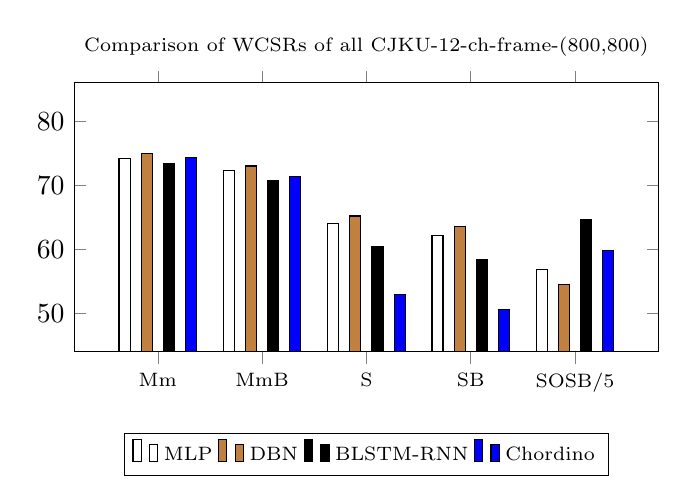
\begin{tikzpicture}
\begin{axis}[
	title={Comparison of WCSRs of all CJKU-12-ch-frame-(800,800)},
	title style = {font=\scriptsize},
    ybar=4pt,
    bar width=4pt,
    enlargelimits=0.2,
        legend style={at={(0.5,-0.3)},
          anchor=north,legend columns=-1},
   % ylabel={WCSR},
    %y label style={font=\scriptsize},
    symbolic x coords={Mm,MmB,S,SB,SOSB/5},
    x tick label style={font=\scriptsize},
    xtick=data,
    ymin=50, ymax=80,
    %nodes near coords,
    %nodes near coords align={vertical},
    legend style={font=\scriptsize},
    ]
\addplot [ybar,fill=white,draw=black] coordinates {(Mm,74.2)(MmB,72.3)(S,64.0)(SB,62.2)(SOSB/5,56.9)};
\addplot [ybar,fill=brown,draw=black] coordinates {(Mm,74.9)(MmB,73.0)(S,65.2)(SB,63.5)(SOSB/5,54.5)};
\addplot [ybar,fill=black,draw=black] coordinates {(Mm,73.3)(MmB,70.8)(S,60.5)(SB,58.4)(SOSB/5,64.7)};
\addplot [ybar,fill=blue,draw=black] coordinates {(Mm,74.3)(MmB,71.4)(S,53.0)(SB,50.6)(SOSB/5,59.8)};
\legend{MLP,DBN,BLSTM-RNN, Chordino}
\end{axis}
\end{tikzpicture}
\caption{Compare the best systems with Chordino. All systems are trained with CJKU-12-ch-frame-(800,800).}
\label{fig:3-compchordino}
\end{figure}

At last some best system representatives are compared with the baseline approach - Chordino. In Figure~\ref{fig:3-compchordino}, there is one representative for each deep learning model, all trained with CJKU-12-ch-frame-(800,800). They are compared with Chordino in terms of five categories: four WCSRs and the versatility measure SOSB.

As shown, these systems all outperform Chordino by a large range in S and SB, and they are fairly comparable with Chordino in Mm and MmB. In terms of versatility, Chordino is not bad at all, outperforming both MLPs and DBN's representatives. But the most well-rounded system is based on BLSTM-RNN, outscoring Chordino by huge amount.

\section{MIREX 2016 Results}
MIREX ACE 2016 features 4 sets of systems implemented by four different groups:
\begin{itemize}
\item CM1: Chordino, from Queen Mary University of London;
\item DK*: features three variants of the ACE approach proposed in this chapter (note that DK4, which is from another design approach, is skipped in the following discussion);
\item FK*: implemented by Korzeniowski and Widmer, featuring the systems in two previous papers \cite{Korzeniowski2016feature,Korzeniowski2016convolutional}
\item KO1: shineChords, a time-frequency reassign approach proposed by Khadkevich and Omologo \cite{khadkevich2011time}.
\end{itemize}

\subsection{Dataset and Vocabulary}
It should be noted that except CM3, whose model parameters are all manually specified, all other systems involve extensive training:
\begin{itemize}
\item KO1's description does not mention its training set, but it is probably trained with the Isophonic dataset (MIREX 2009 set) \cite{burgoyne2014comparative}. This can be easily spot by simply noticing that, compared with other systems, it has too high a SB score in Isophonic, while not as high in other test sets.

\item FK* are trained with the Isophonic, Robbie Williams\footnote{\url{https://www.researchgate.net/publication/260399240\_Chord\_and\_Harmony\_annotations\_of\_the\_first\_five\_albums\_by\_Robbie\_Williams}}, RWC and the public part of McGill Billboard\footnote{\url{http://ddmal.music.mcgill.ca/billboard}} dataset.

\item DK* are trained with USPop and RWC dataset. Note that they do not contain any test set in MIREX ACE 2016.
\end{itemize}

In terms of chord vocabulary, both DK3, FK* and KO1 only support majmin, CM1 supports a large vocabulary including most types in SeventhsBass, and DK1\&2 support exactly the SeventhsBass.

\begin{table*}[htb]
\centering
\scriptsize
\caption{MIREX 2016 Results. B = Bass, Mm = MajMin, MmB = MajMinBass, R = Root, S = Sevenths, SB = SeventhsBass, Seg = Segmentation Quality}
\label{tab:3-mirex2016}
\begin{tabular}{|c|c|c|c|c|c|c|c|c|}\hline
Algorithm & R & Mm & MmB & S & SB & Seg & UnderSeg & OverSeg \\ \hline
Isophonics 2009\\ \hline
CM1 & 78.56 & 75.41 & 72.48 & 54.67 & 52.26 & 85.90 & 87.17 & 86.09\\ \hline
DK1 & 79.21 & 76.19 & 74.00 & 66.02 & 64.15 & 85.71 & 82.62 & 91.23\\ \hline
DK2 & 77.84 & 74.49 & 71.93 & 61.61 & 59.47 & 85.82 & 82.72 & 91.28\\ \hline
DK3 & 80.03 & 77.55 & 74.79 & 68.40 & 65.88 & 85.81 & 82.50 & 91.53\\ \hline
DK4 & 76.05 & 72.96 & 71.41 & 62.77 & 61.44 & 78.19 & 87.97 & 72.43\\ \hline
FK2 & 86.09 & 85.53 & 82.24 & 74.42 & 71.54 & 87.76 & 85.79 & 90.73\\ \hline
FK4 & 82.28 & 80.93 & 78.03 & 70.91 & 68.26 & 85.62 & 82.40 & 90.89\\ \hline
KO1 & 82.93 & 82.19 & 79.61 & 76.04 & 73.43 & 87.69 & 85.66 & 91.24\\ \hline
Billboard 2012 \\ \hline
CM1 & 74.15 & 72.22 & 70.21 & 55.35 & 53.40 & 83.64 & 85.31 & 83.39\\ \hline
DK1 & 75.28 & 73.57 & 71.87 & 59.98 & 58.53 & 83.35 & 80.26 & 88.52\\ \hline
DK2 & 73.77 & 71.69 & 69.86 & 58.66 & 57.00 & 83.57 & 80.40 & 88.70\\ \hline
DK3 & 75.92 & 74.75 & 72.69 & 53.42 & 51.67 & 83.39 & 79.97 & 88.92\\ \hline
DK4 & 72.59 & 70.85 & 69.78 & 56.29 & 55.36 & 76.13 & 87.72 & 70.05\\ \hline
FK2 & 85.64 & 85.38 & 82.55 & 60.70 & 58.38 & 87.62 & 86.09 & 90.13\\ \hline
FK4 & 79.23 & 78.62 & 76.20 & 56.53 & 54.51 & 85.09 & 81.98 & 89.94\\ \hline
KO1 & 77.45 & 75.58 & 73.51 & 57.68 & 55.82 & 84.16 & 82.80 & 87.44\\ \hline
Billboard 2013 \\ \hline
CM1 & 71.16 & 67.28 & 65.20 & 48.99 & 47.17 & 81.54 & 83.11 & 82.63\\ \hline
DK1 & 72.06 & 68.69 & 67.26 & 54.54 & 53.29 & 80.82 & 77.58 & 88.06\\ \hline
DK2 & 70.18 & 66.54 & 64.66 & 52.97 & 51.41 & 80.85 & 77.68 & 88.02\\ \hline
DK3 & 72.39 & 68.53 & 66.55 & 48.99 & 47.28 & 80.76 & 77.26 & 88.30\\ \hline
DK4 & 69.56 & 65.83 & 64.78 & 51.81 & 50.93 & 74.55 & 86.31 & 69.18\\ \hline
FK2 & 80.07 & 77.89 & 75.42 & 55.41 & 53.22 & 82.94 & 82.43 & 86.80\\ \hline
FK4 & 74.66 & 71.85 & 69.44 & 51.93 & 49.80 & 80.61 & 77.19 & 88.70\\ \hline
KO1 & 75.36 & 71.39 & 69.43 & 53.57 & 51.78 & 81.63 & 79.61 & 87.75\\ \hline
JayChou 2015 \\ \hline
CM1 & 72.75 & 72.08 & 65.48 & 54.39 & 48.98 & 86.60 & 86.89 & 86.91\\ \hline
DK1 & 74.70 & 73.87 & 70.33 & 54.98 & 52.25 & 86.76 & 82.78 & 91.79\\ \hline
DK2 & 72.19 & 72.55 & 69.10 & 54.09 & 51.46 & 87.09 & 83.35 & 91.75\\ \hline
DK3 & 75.01 & 74.75 & 63.56 & 49.27 & 40.24 & 86.76 & 82.54 & 92.08\\ \hline
DK4 & 71.51 & 69.03 & 65.93 & 50.07 & 47.45 & 78.11 & 87.87 & 70.56\\ \hline
FK2 & 79.51 & 78.66 & 68.15 & 50.69 & 42.34 & 86.81 & 85.43 & 88.56\\ \hline
FK4 & 76.13 & 75.44 & 64.36 & 49.69 & 40.74 & 84.55 & 81.22 & 88.95\\ \hline
KO1 & 78.73 & 77.69 & 66.87 & 54.16 & 44.55 & 88.46 & 87.12 & 90.11\\ \hline
RobbieWilliams 2016 \\ \hline
CM1 & 81.90 & 78.25 & 76.05 & 57.92 & 55.90 & 87.96 & 88.96 & 87.45\\ \hline
DK1 & 81.50 & 77.77 & 76.10 & 68.88 & 67.34 & 87.03 & 83.22 & 92.11\\ \hline
DK2 & 79.01 & 75.97 & 73.57 & 65.26 & 62.98 & 87.20 & 83.40 & 92.23\\ \hline
DK3 & 81.85 & 78.56 & 76.16 & 74.71 & 72.55 & 86.98 & 82.95 & 92.34\\ \hline
DK4 & 78.92 & 75.15 & 73.66 & 66.72 & 65.34 & 81.82 & 88.44 & 76.88\\ \hline
FK2 & 88.53 & 87.23 & 84.19 & 82.57 & 79.88 & 90.04 & 88.62 & 91.88\\ \hline
FK4 & 83.37 & 80.96 & 78.42 & 77.04 & 74.76 & 87.22 & 84.50 & 91.02\\ \hline
KO1 & 83.55 & 80.33 & 78.16 & 73.54 & 71.39 & 88.04 & 85.39 & 91.68\\ \hline
\end{tabular}
\end{table*}
\subsection{Results and Discussions}
Table~\ref{tab:3-mirex2016} shows the results of MIREX ACE 2016. Within the context of this thesis, the main focus of the results is the SeventhsBass column.

In Isophonic test, KO1 gets the highest score. But this is probably because of its over-fitting the data, as explained previously, that it actually scores much lower in tests that it does not previously know, such as JayChou 2015. Both FK2 and FK4 come next to KO1, but unfortunately they are all informed with this test set. Since it is not clear to what extend the systems over-learn the data, the results of this test is not statistically valid to deduce any reasonable conclusions regarding these systems.

In Billboard 2012 and 2013 tests, the best performances are both from DK1. Although FK* learn from part of the test set, they somehow does not outperform DK1. Moreover, DK1 outscore KO1 by about 3 points in both tests, which demonstrates a better generalization capability in DK1 system.

JayChou 2015 test is probably the most convincing one, since on one had none of the systems are learning this set, and on the other hand it has more than 20\% of chords other than maj, min and sevenths, much more than other test sets. The performance on this test could well demonstrate the system's vocabulary versatility. This can be noticed by making comparison within the DK* systems, where DK1 and DK2 perform much better than DK3 in SB. The best two systems in this test are DK1 and DK2, outscoring the FK* systems by around 10 points, and the KO1 system by about 8 points.

Robbie Williams test somehow shows the reverse ranking of JayChou 2015. DK3 leads both DK1 and DK2 by about 5 and 10 points. FK* are the best performing ones, but unfortunately they might over-learn the data. It is interesting to note that KO1 scores 71.39, slightly less that DK3's 72.55. This strongly indicates that this test is mainly composed of maj, min and sevenths (probably >90\%), which is very similar to the chord composition of the Isophonic set. Therefore systems that only support a small chord vocabulary will have a huge advantage by not being able to have confusions on long-tail chords.

\section{On Smaller Vocabulary}
This chapter is mainly developed based on large vocabulary, specifically, the SeventhsBass vocabulary. In order to do a comparison between the proposed system framework and other approaches, a set of experiments are conducted using two smaller vocabularies: 1, MajMin; 2, Full121 vocabulary introduced by Mauch \cite{mauch2010automatic} (also mentioned in Section~\ref{sec:2-largevocab}). For MajMin system implementation, each label in the training set will be mapped to its MajMin form following a normal mapping scheme \cite{harte2010towards,pauwels2013evaluating}. As a result, each deep learning model will be trained on a dataset with only MajMin labels. For Full121 implementation, a slightly modified version of chord mapping strategy \cite{mauch2010automatic} is followed.

\subsection{On MajMin}
Table~\ref{tab:3-overallres} shows a SeventhsBass evaluation comparison, where all systems, except for Chordino, only supports MajMin vocabulary. The results show that on one hand the overall performances of these systems are only fairly comparable with those in Section~\ref{sec:3-p9}, on the other hand the SOSB of these systems are all much lower because of a much smaller vocabulary than Chordino.
\begin{table}[h]
\footnotesize
\centering
\caption{Overall WCSR scores; All systems are trained with CJKUR-(800,800), with only MajMin vocabulary support.}
\label{tab:3-overallres}
\begin{tabular}{|c|c|c|c|c|c|c|c|c|}\hline
System & B & Mm & MmB & R & S & SB & Seg & SOSB \\ \hline
chordino & 76.41 & 74.30 & 71.40 & 77.19 & 52.99 & 50.60 & 83.87 & 299.01\\ \hline
MLP-ch & 74.71 & 73.25 & 71.22 & 75.74 & 65.08 & 63.18 & 83.57 & 151.57\\ \hline
DBN-ch & 77.04 & 75.50 & 73.39 & 78.10 & 67.26 & 65.30 & 83.78 & 156.80\\ \hline
BLSTM-RNN-ch & 76.88 & 75.05 & 72.84 & 78.11 & 66.58 & 64.50 & 83.74 & 157.46\\ \hline
MLP-ns & 72.65 & 70.00 & 68.14 & 73.35 & 62.72 & 60.98 & 83.59 & 140.57\\ \hline
DBN-ns & 72.91 & 70.96 & 69.14 & 73.66 & 63.33 & 61.66 & 83.44 & 144.89\\ \hline
BLSTM-RNN-ns & 76.04 & 73.98 & 71.99 & 76.85 & 65.85 & 64.03 & 83.76 & 153.63\\ \hline
\end{tabular}
\end{table}

Table~\ref{tab:3-detailres} shows the SeventhsBass categorical breakdown. Take DBN-ch as representative, since it only supports MajMin, its $maj$ and $min$ scores are much higher than the Chordino's. As the two chord types comprise of the majority of the data set population, that's why it has a much higher SB score. However, by relaxing the evaluation strength from SB to Mm, the performance difference between DBN-ch and Chordino becomes less and less.

\begin{landscape}
\thispagestyle{plain}
\begin{table*}[h]
\scriptsize
\caption{Detail SeventhsBass WCSR scores. All systems are trained with CJKUR-(800,800), with only MajMin vocabulary support. M = Major, m = minor, N = no chord. The \%B row shows the composition of chords in the test dataset.}
\label{tab:3-detailres}
\begin{tabular}{|c|c|c|c|c|c|c|c|c|c|c|c|c|c|c|c|c|c|c|c|}\hline
\%B & 2.01 & 0.95 & 63.31 & 0.02 & 0.17 & 0.27 & 0.82 & 0.08 & 0.06 & 0.39 & 8.33 & 0.61 & 0.44 & 14.99 & 0.01 & 0.06 & 0.41 & 2.37 & 4.63\\ \hline
 & M/5 & M/3 & M & M7/5 & M7/3 & M7/7 & M7 & 7/5 & 7/3 & 7/b7 & 7 & m/5 & m/b3 & m & m7/5 & m7/b3 & m7/b7 & m7 & N\\ \hline
chordino & 19.9 & 17.1 & 54.4 & 0.0 & 0.0 & 0.0 & 55.6 & 0.0 & 0.0 & 5.7 & 41.0 & 0.0 & 0.0 & 54.3 & 0.0 & 0.0 & 0.0 & 51.0 & 2.2\\ \hline
MLP-ch & 0.0 & 0.0 & 77.6 & 0.0 & 0.0 & 0.0 & 0.0 & 0.0 & 0.0 & 0.0 & 0.0 & 0.0 & 0.0 & 74.0 & 0.0 & 0.0 & 0.0 & 0.0 & 2.8\\ \hline
DBN-ch & 0.0 & 0.0 & 80.0 & 0.0 & 0.0 & 0.0 & 0.0 & 0.0 & 0.0 & 0.0 & 0.0 & 0.0 & 0.0 & 76.8 & 0.0 & 0.0 & 0.0 & 0.0 & 3.0\\ \hline
BLSTM-RNN-ch & 0.0 & 0.0 & 79.3 & 0.0 & 0.0 & 0.0 & 0.0 & 0.0 & 0.0 & 0.0 & 0.0 & 0.0 & 0.0 & 78.2 & 0.0 & 0.0 & 0.0 & 0.0 & 2.5\\ \hline
MLP-ns & 0.0 & 0.0 & 76.4 & 0.0 & 0.0 & 0.0 & 0.0 & 0.0 & 0.0 & 0.0 & 0.0 & 0.0 & 0.0 & 64.2 & 0.0 & 0.0 & 0.0 & 0.0 & 2.9\\ \hline
DBN-ns & 0.0 & 0.0 & 76.3 & 0.0 & 0.0 & 0.0 & 0.0 & 0.0 & 0.0 & 0.0 & 0.0 & 0.0 & 0.0 & 68.6 & 0.0 & 0.0 & 0.0 & 0.0 & 2.9\\ \hline
BLSTM-RNN-ns & 0.0 & 0.0 & 79.0 & 0.0 & 0.0 & 0.0 & 0.0 & 0.0 & 0.0 & 0.0 & 0.0 & 0.0 & 0.0 & 74.7 & 0.0 & 0.0 & 0.0 & 0.0 & 2.7\\ \hline
\end{tabular}
\end{table*}
\end{landscape}

\subsection{On Full121}

\begin{table}[h]
\footnotesize
\centering
\caption{Full121 WCSR scores. Tested on TheBeatles180 dataset (180 tracks out of the 216 tracks Isophonic 2009) All systems are trained with CJKUR-(800,800)-ch, with Full121 vocabulary support.}
\label{tab:3-full}
\begin{tabular}{|c|c|c|}\hline
System & Full121 WCSR & Seg \\ \hline
MLP & 73.43 & 83.77 \\ \hline
DBN & 75.46 & 83.92 \\ \hline
BLSTM-RNN & 73.63 & 83.80 \\ \hline
\end{tabular}
\end{table}

\begin{table}[h]
\footnotesize
\centering
\caption{Full121 scores. Tested on Isophonic 2009 dataset with 3-fold cross-validation\cite{ni2012end}}
\label{tab:3-fullhp}
\begin{tabular}{|c|c|c|}\hline
System & Full121 Chord Precision (CP) & Seg \\ \hline
CH(Chordino) & 50.31 & N/A \\ \hline
HP(Harmonic Analyzer) & 70.26 & N/A\\ \hline
\end{tabular}
\end{table}

\begin{table}[h]
\footnotesize
\centering
\caption{Full121 scores. Tested on Isophonic 2009 dataset with 5-fold cross-validation \cite{mauch2010automatic}}
\label{tab:3-fullmbk}
\begin{tabular}{|c|c|c|}\hline
System & Full121 Relative Correct Overlap (RCO) & Seg \\ \hline
trained MBK & 41.8 & N/A \\ \hline
MBK & 56.7 & 77.9 \\ \hline
MBK-NNLS & 61.8 & N/A \\ \hline
\end{tabular}
\end{table}

Table~\ref{tab:3-full} shows results of Full121 vocabulary with the same test set. Table~\ref{tab:3-fullhp} and ~\ref{tab:3-fullmbk} shows Full121 scores by other systems using a slightly larger 216-track test set, which includes the 180-track test set used throughout this chapter. Table~\ref{tab:3-fullhp} is reported in a 3-fold cross-validation manner, while Table~\ref{tab:3-fullhp} is in 5-fold. According to the descriptions \cite{ni2012end,mauch2010automatic}, the computation processes of both CP and RCO metrics are essentially similar to that of WCSR, and they only accept ``exact chord match'' under the vocabulary.

It is difficult to make any conclusive statement out of these three different tables, from slightly different test sets, and reported in different ways. But it is reasonably fair to say that the proposed system framework is not bad at all in handling the Full121 vocabulary.


\section{Summary} \label{sec:3-concln}
This chapter presents an in-depth discussion of a hybrid GMM-HMM-DNN ACE approach. The study is motivated by the current research gap in LVACE, and a general negligence of segmentation-classification isolation. This serves as the basis for chord inversions supportable large vocabulary segmentation-classification ACE system implementation. This chapter then introduces the GMM-HMM-DNN system framework, which leverages handcrafted feature extraction and segmentation processes, and plugs in various deep neural networks to classify the chord within each segment. The design and implementation are guided by systematically sampling and evaluating the design space of the framework.

The results indicate that among the three proposed deep learning models, BLSTM-RNN is the most musically correct and balanced one for practical use.  With more training data, MLP and DBN tends to over-fit the most ordinary chords, but BLSTM-RNN will gradually generalize better in all categories.

It extends naturally from this study that ACE systems should try to focus more on improving long-tail recognition accuracies. That is, instead of considering the overall WCSR of a large vocabulary, attention should also be given to the versatility metric, such as SOSB, or ``Average individual chord accuracy'' \cite{cho2014improved} that summarize scores of every chord type without weighting their populations. Although BLSTM-RNN model is very promising in handling large vocabulary with inversions, developing new methods to train the network in such ``imbalanced class population '' scenario \cite{chawla2004editorial} will undeniably be an important direction that are yet to be explored.

It should be pointed out that the ultimate goal of ACE is to device a computer program that comes as close as possible to human musician's ability to chord transcription. Differentiating between long-tail chords and ordinary chords is undoubtedly what differentiates a musician from an amateur. Now that there are already good systems that match an amateur level \cite{ni2013understanding}, it is a good moment to start to pursuit systems at musician level.

Finally, a piece of timed chord sequence output can be combined with the \textit{.lrc} file\footnote{\url{https://en.wikipedia.org/wiki/LRC\_(file\_format)}} of the same track to become a chord-lyrics sheet, which is one of the most frequently used pop music sheet formats. This combination process is implemented\footnote{\url{https://github.com/tangkk/songtranspose}} by the author of this thesis. Figure~\ref{fig:3-aihenjiandan} shows an example chord-lyrics output.
\begin{figure}[h]
    \centering
        \includegraphics[width=0.8\columnwidth]{3/figures/aihenjiandan.pdf}
    \caption{Chord-lyrics output of \textit{Aihenjiandan} (by Taiwan singer-songwriter David Tao)}
    \label{fig:3-aihenjiandan}
\end{figure}
Note that in this case the lyrics might not be perfectly aligned with chords, since an \textit{.lrc} file only has information on the start and end time of each lyrics line, rather than each word. A more sophisticated solution would be to use audio-lyrics alignment tool \cite{mauch2010lyrics} as a preprocessing stage before matching the lyrics and chords.


% ---------------------------------------------------------------------------
%: ----------------------- end of thesis sub-document ------------------------
% ---------------------------------------------------------------------------

